\documentclass[12pt,a4paper]{report}
\usepackage[utf8]{inputenc}
\usepackage[english]{babel}
\usepackage{amsmath}
\usepackage{amsfonts}
\usepackage{amssymb}
\usepackage{graphicx}
\usepackage{eurosym}
\usepackage[left=2cm,right=2cm,top=2cm,bottom=2cm]{geometry}
\usepackage{wrapfig}
\usepackage{mathdots}
\usepackage{caption}
\usepackage{cite}
\usepackage{mathrsfs}
\usepackage{float}
\usepackage[]{mcode}

\author{Communications department}
\title{Ground Station localization}

\begin{document}
\maketitle
\tableofcontents
\listoffigures

\chapter*{Aim of the document}
\paragraph{}
Until now, it has been talked about the Ground Stations independently of wherever they are. It has to be studied where to place the Ground Stations in order to optimize the Ground Segment performance. This decision will depend mainly of the constellation characteristics, the earth topography and the country legislation and resources. 
\paragraph{}
This report will collect the analysis and procedures for arriving to the final decision of where the Ground Stations would be placed.

\chapter{Coverage analysis}
\section{Aim} 
\paragraph{}
Given the constellation topology, it will be studied the coverage of a Ground Station depending on its longitude and latitude. The aim of this analysis is to show where a Ground Station would have more coverage and propose a first approximation and proposal of the 3 Ground Station placement.

\section{Method}
For this porpoise it is developed a Matlab algorithm which which calculates, in a given moment, how many satellites can see an make contact a Ground Station in a given place of the earth. It has to be said that this analysis must be done during time since the satellites and the Earth are constantly moving. For doing that the algorithm follows the steps below:
\begin{enumerate}
\item Calculate where the satellites are refereed to an inertial Cartesian coordinates system, with the origin at the center of the Earth. This state analysis its done for a several time period with an adequate time-step. 
\item Calculate the Ground Station position refereed to the mentioned system. Since the system is inertial, the Ground Station will describe a circle in the rotational plane of the Earth relative to this system. This trajectory depend on the latitude and longitude of the place. This position is calculated for the same time period.
\item Calculate, for each time step, how many links can the station make. It will depend on the angle between the station and every satellite, and also the minimum elevation angle. 
\end{enumerate}
\paragraph{}
After seeing reasonable results modifying the parameters of the constellation and of the Ground station, the algorithm is verified simulating the Iridium constellation. Entering the parameters of this system, the results verifies the algorithm
\paragraph{}
Once this algorithm is tested and verified, it is studied the links during the day for several longitudes and latitudes and how this parameters affect to the coverage of the station.
\paragraph{}
The code used can be found at the annexes 1 to 4.

\section{Latitude analysis}
\paragraph{}
It is easy to see that the latitude changing effect is practically independent for the longitude. For this reason, it is studied the links during the day for a given longitude. 
\paragraph{}
Doing the analysis for latitudes between 0º and 90º during 2 days, with a 5 minutes time-step, this are the results:

\begin{figure}[H]
\begin{center}
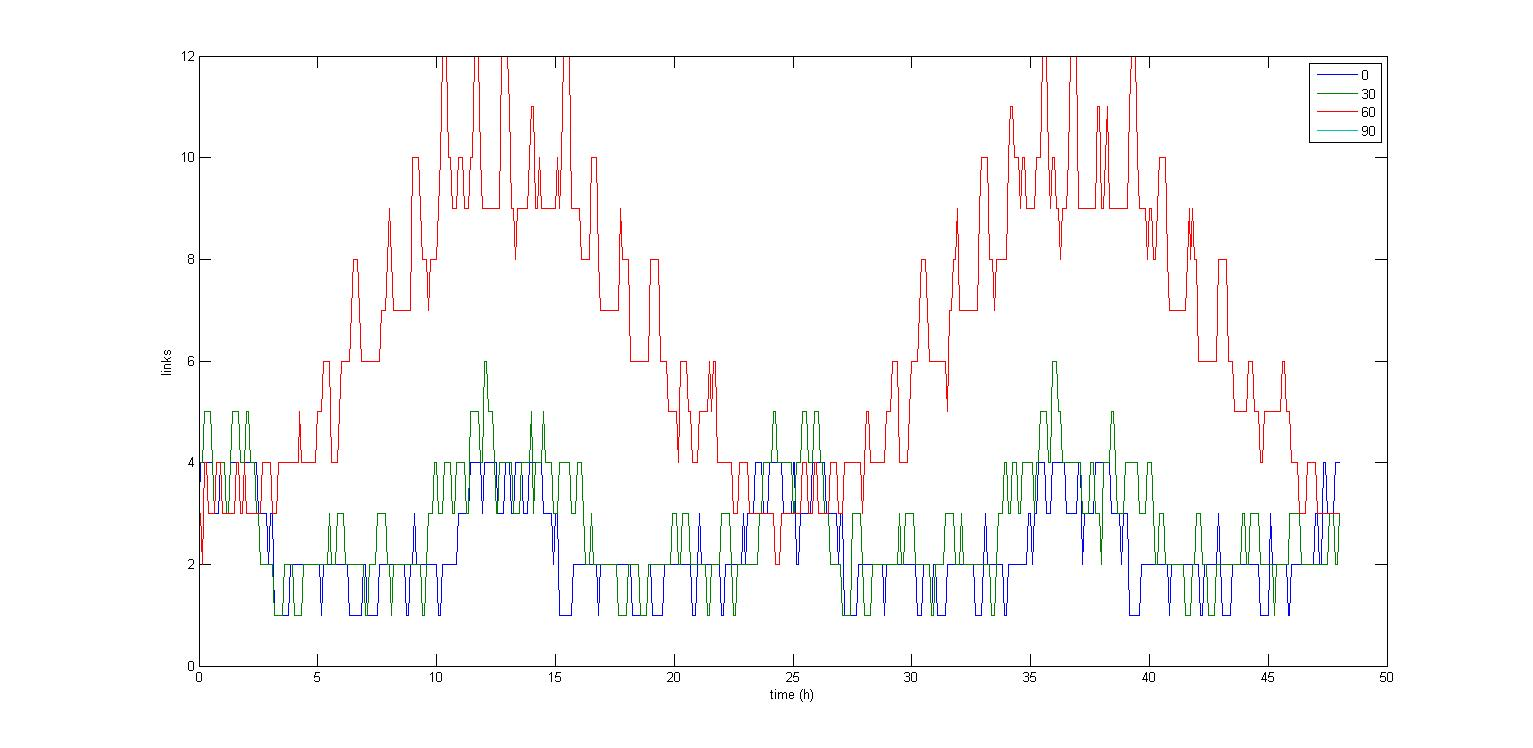
\includegraphics[scale=0.30]{0_30_90_lat.jpg}
\caption{Links vs time for latitudes from 0º to 90º}
\end{center}
\end{figure}

\paragraph{}
At it is shown in the figure 1.1 the behaviour is not constant during the day. For every day there is a peak and a valley. This is produced for the cylindrical asymmetry of the constellation. It is also seen that at the pole there is not any coverage at all. It was considered and assumed at the design of the constellation since it does involves any problem at the performance of the system. It is also seen that for a equatorial latitude there is always 1 link at least. The equator is the most critical place because is where de satellites of one plane to the others are more separated. For this reason, it can be ensured global coverage except at the pole. Finally it is significant that at higher latitudes there is better coverage.
\paragraph{}
Doing the same for negative latitudes the following results are obtained:

\begin{figure}[H]
\begin{center}
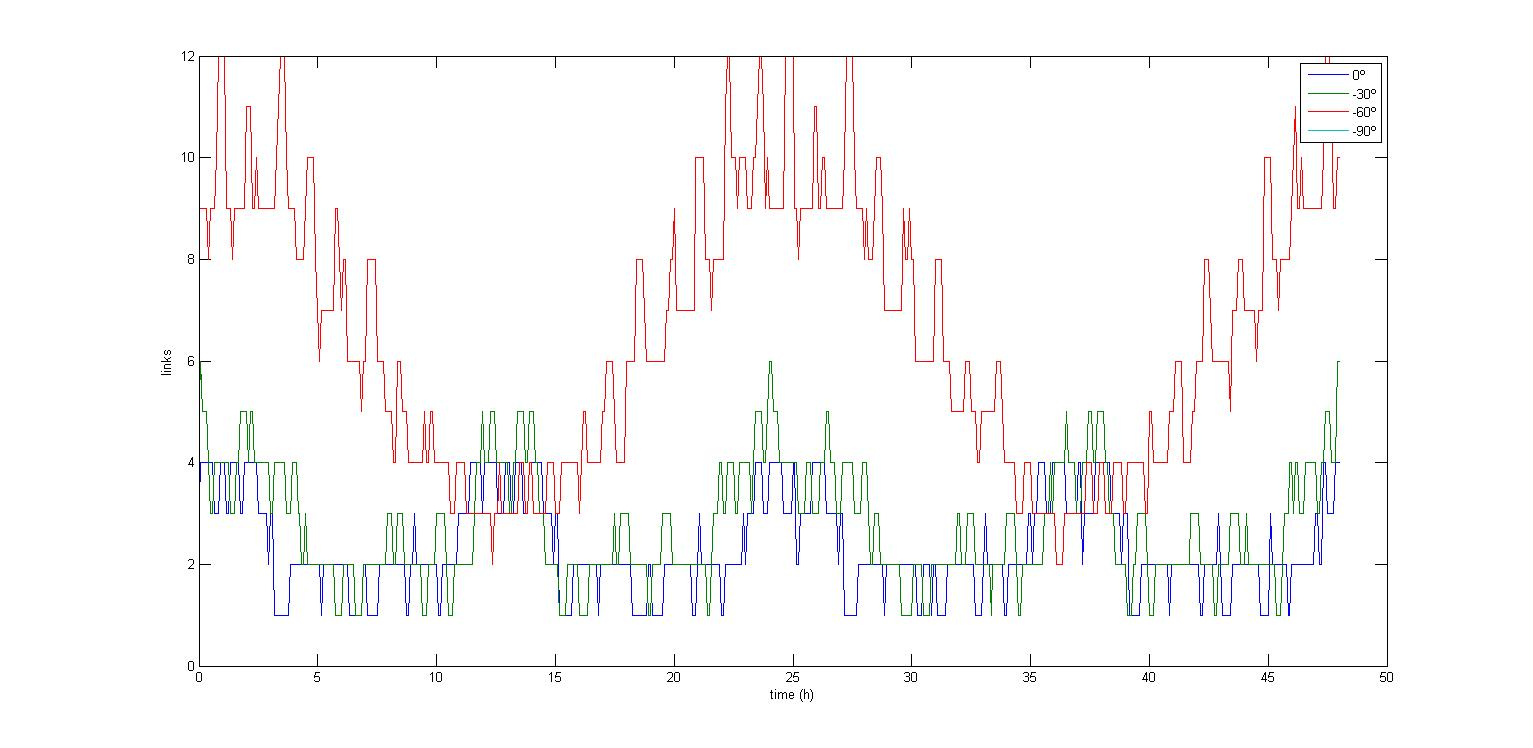
\includegraphics[scale=0.30]{0_-30_-90_lat.jpg}
\caption{Links vs time for latitudes from 0º to -90º}
\end{center}
\end{figure}

\paragraph{}
Comparing the results of the figure 1.2 with the figure 1.1 it is seen that they are practically the same with an offset of 12 hours. They are also seen small local deviations, but these are not much significant because of the time-step. This time-step is of 5 minutes for a first sight of the tendencies, and it do not allow extremely precise results.
\paragraph{}
Taking in account that the results of positive latitudes can be extrapolated to negative ones, the rest of the analysis is done for positive latitudes. At this point, it has to be found from which latitude, over 60º, it begins to lose the coverage.

\begin{figure}[H]
\begin{center}
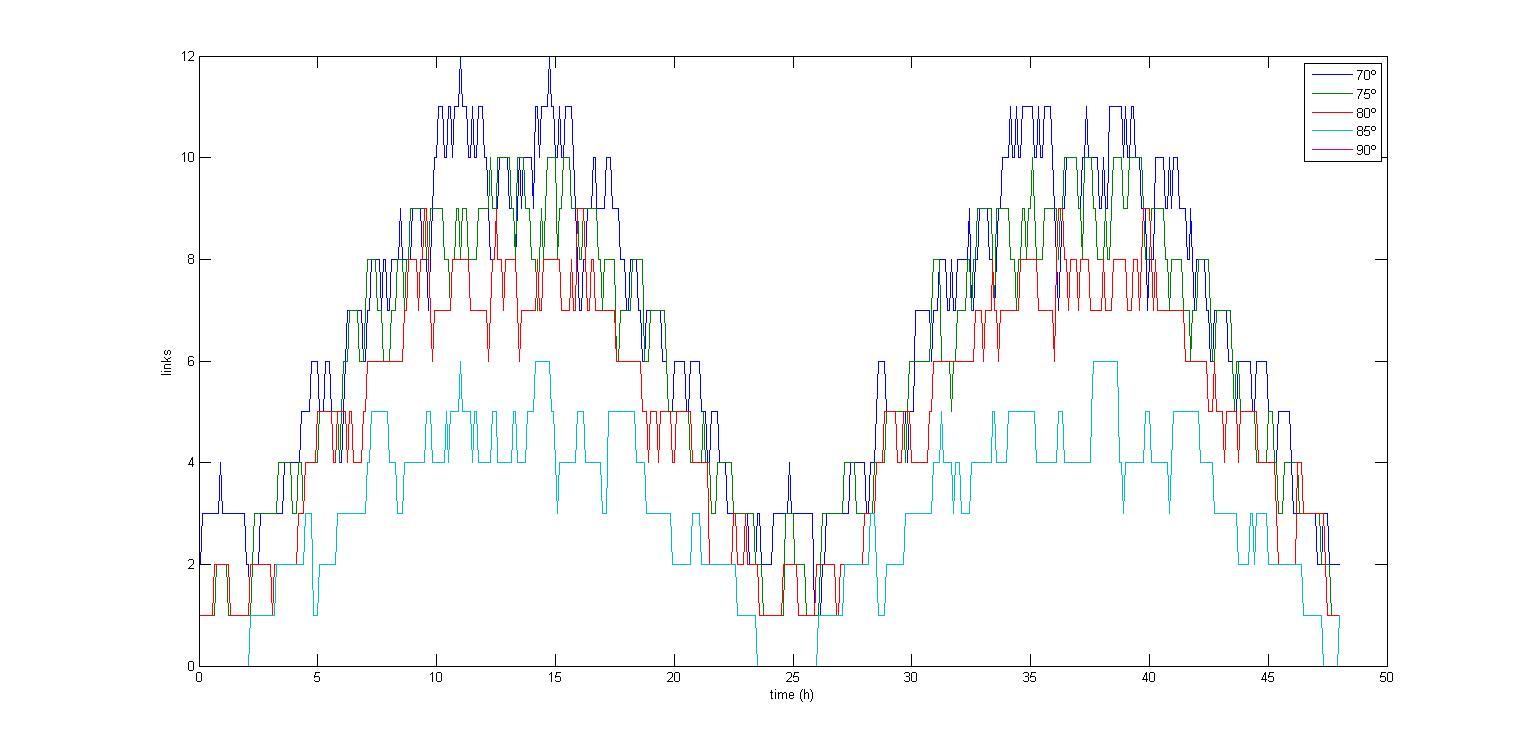
\includegraphics[scale=0.30]{70_5_90_lat.jpg}
\caption{Links vs time for latitudes from 70º to 90º}
\end{center}
\end{figure}

\paragraph{}
It is seen that over 80º of latitude the system starts to lose coverage. It does not case any problem because there are not inhabited zones over +80º or under -80º. For situating the Ground Stations it has to be considered this restriction.
\paragraph{}
For situating the stations, it is studied which latitudes provides higher coverage. As it is seen in figure 1.1 it should be around 60º.

\begin{figure}[H]
\begin{center}
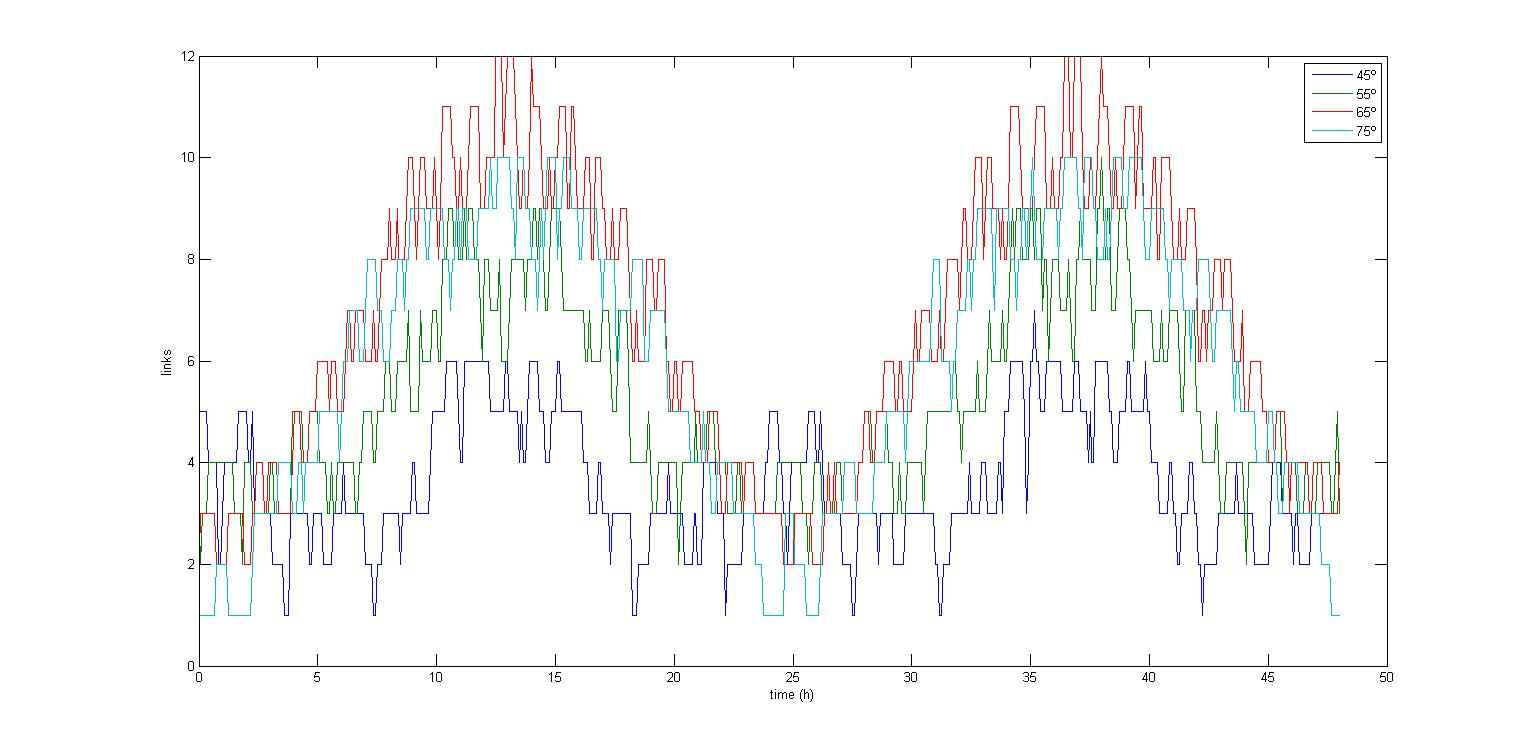
\includegraphics[scale=0.30]{45_10_75_lat.jpg}
\caption{Links vs time for latitudes from 45º to 75º}
\end{center}
\end{figure}

\paragraph{}
As it can be seen in the figure 1.4 the optimal latitude must be between 55º and 75º. Expanding the analysis:

\begin{figure}[H]
\begin{center}
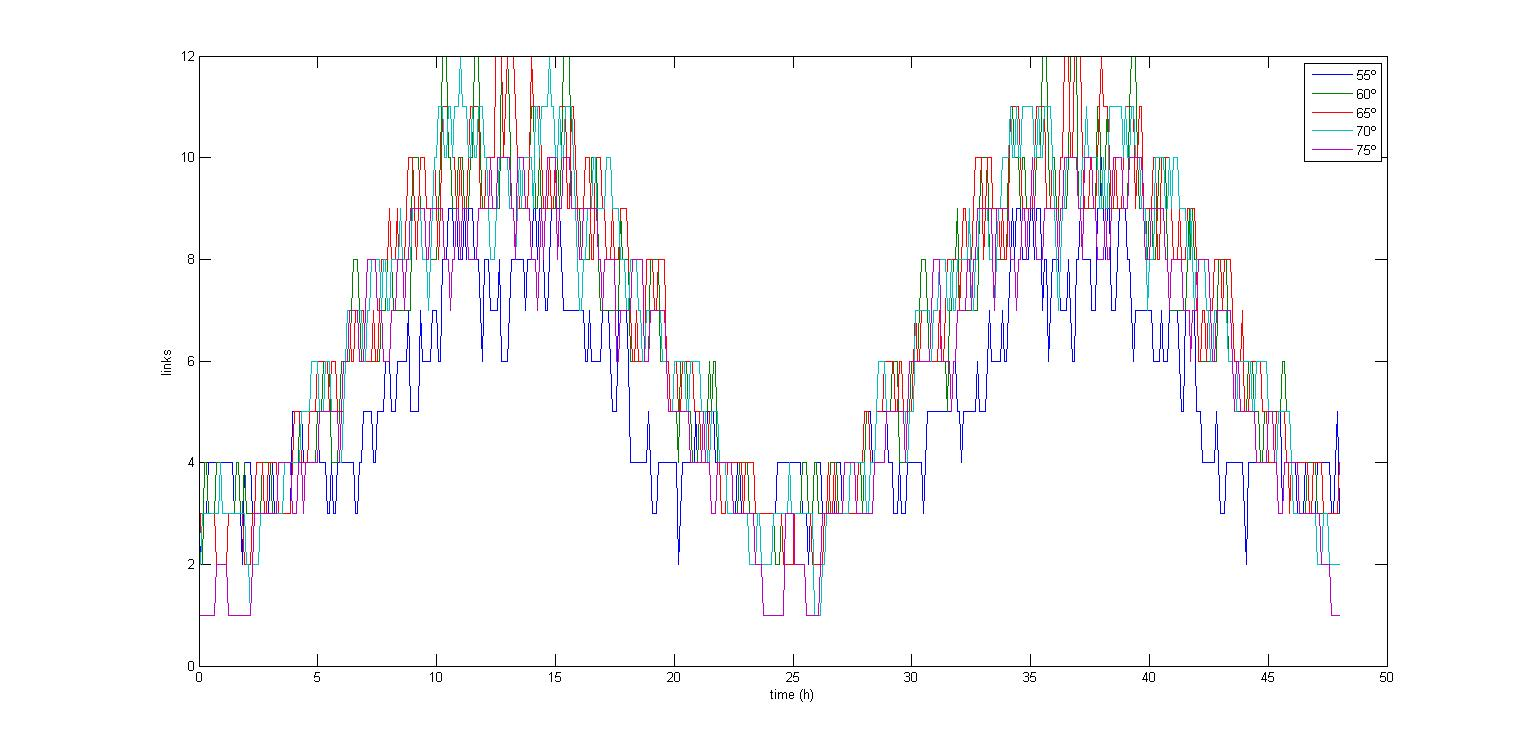
\includegraphics[scale=0.30]{55_5_75_lat.jpg}
\caption{Links vs time for latitudes from 55º to 75º}
\end{center}
\end{figure}

\paragraph{}
The better performance is registered around 60º and 65º. Extending a little more the analysis:

\paragraph{}
The figure 1.5 suggest that between 50º and 60º there is always at least 1 link. But looking it carefully, at the hour 37, there is a local deviation to 0 links. This requires a more accurate analysis decreasing the time-step. For 30 seconds time-step:

\begin{figure}[H]
\begin{center}
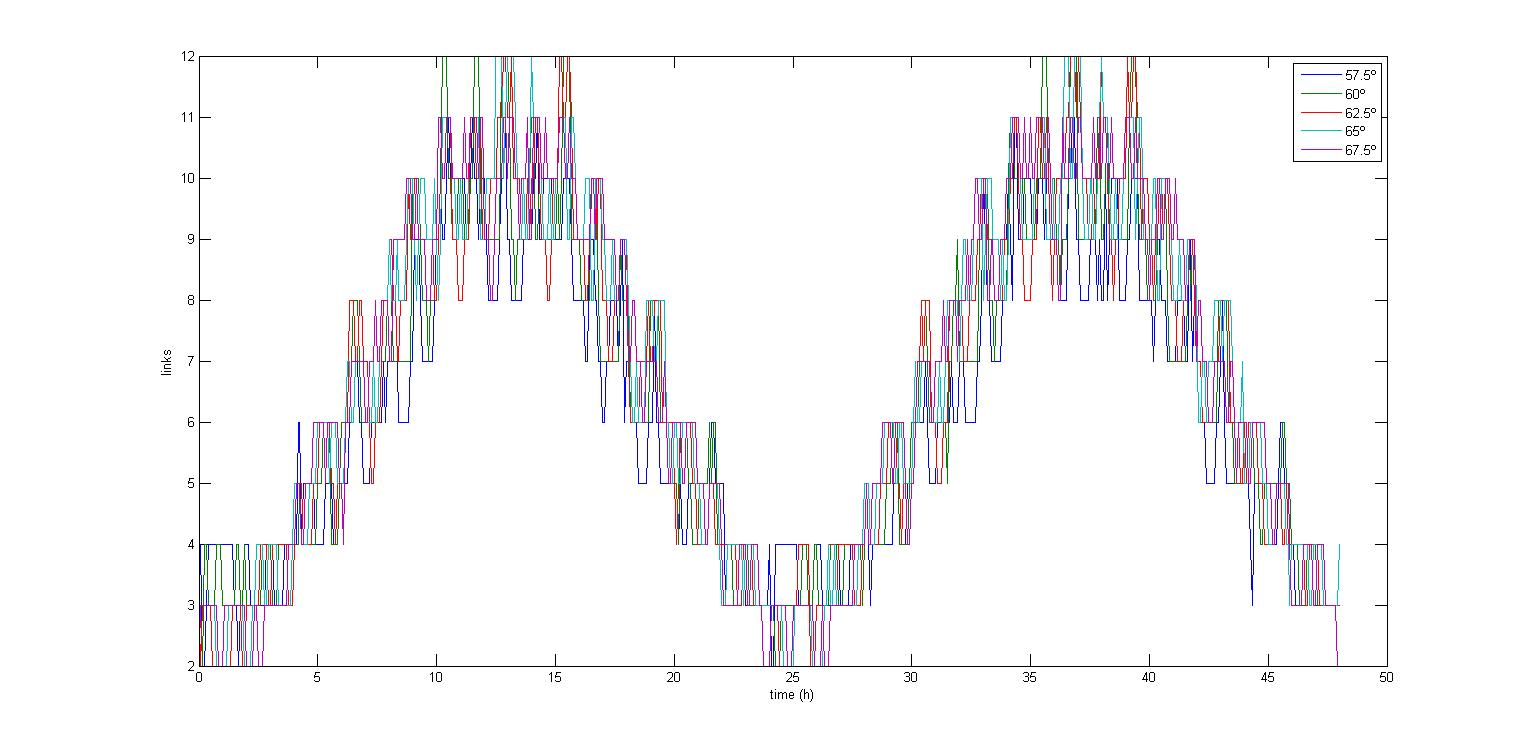
\includegraphics[scale=0.30]{575_25_675_lat.jpg}
\caption{Links vs time for latitudes from 57.5º to 67.5º}
\end{center}
\end{figure}

\paragraph{}
There is any significant different coverage in the range analysed in the figure 1.6. For ensuring the results, and avoid possible loses of link locally in time, it is analysed the same range with a lower time-step.


\begin{figure}[H]
\begin{center}
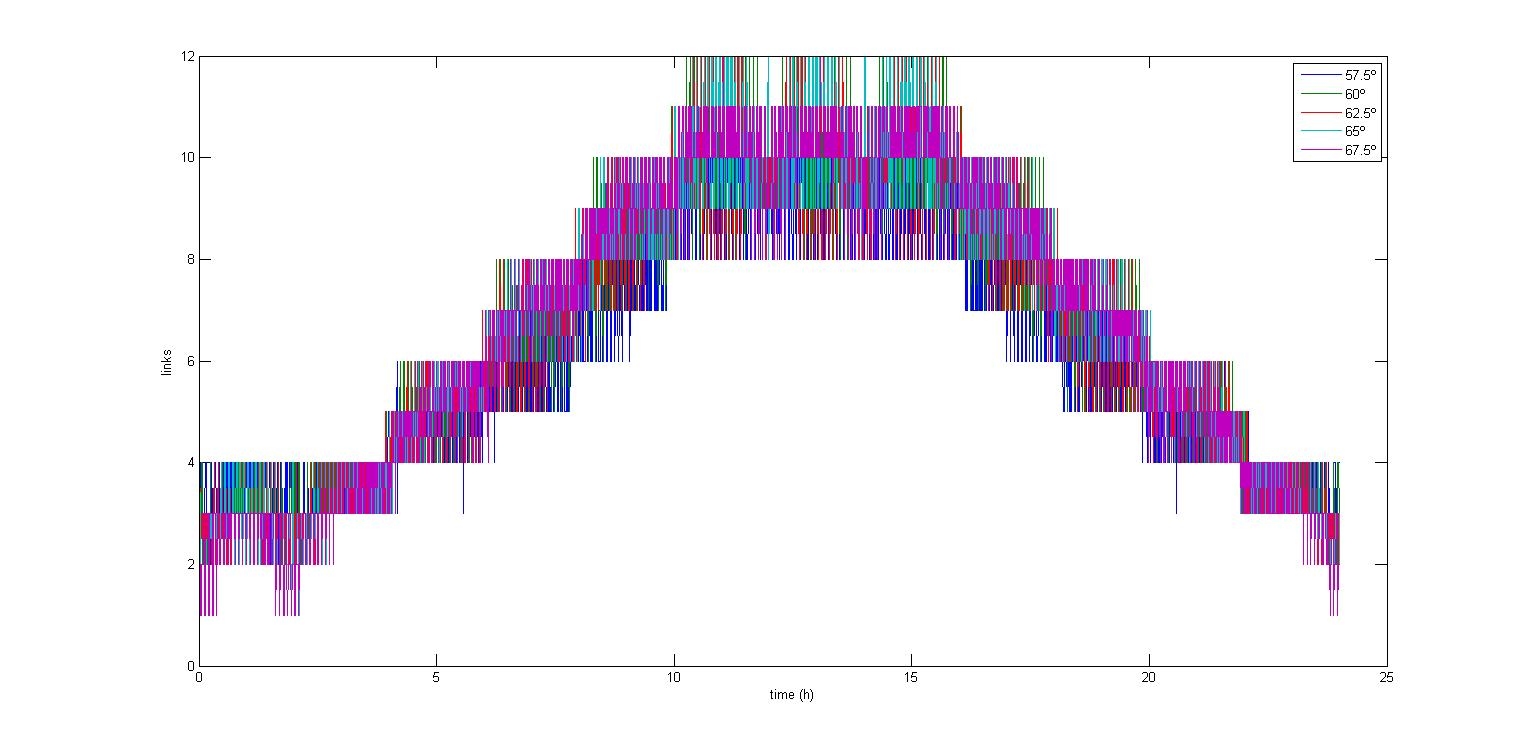
\includegraphics[scale=0.30]{575_25_675_(30s)_lat.jpg}
\caption{Links vs time for latitudes from 57.5º to 67.5º with 30 seconds time-step}
\end{center}
\end{figure}

\paragraph{}
It is seen that between 65º and 67.5º the system loses the 2nd link and for a wile the station would be connected only to 1 satellite. It is optimum to place the stations between +57.5º and +62.5º of latitude. For verifying the results for the opposite latitudes:

\begin{figure}[H]
\begin{center}
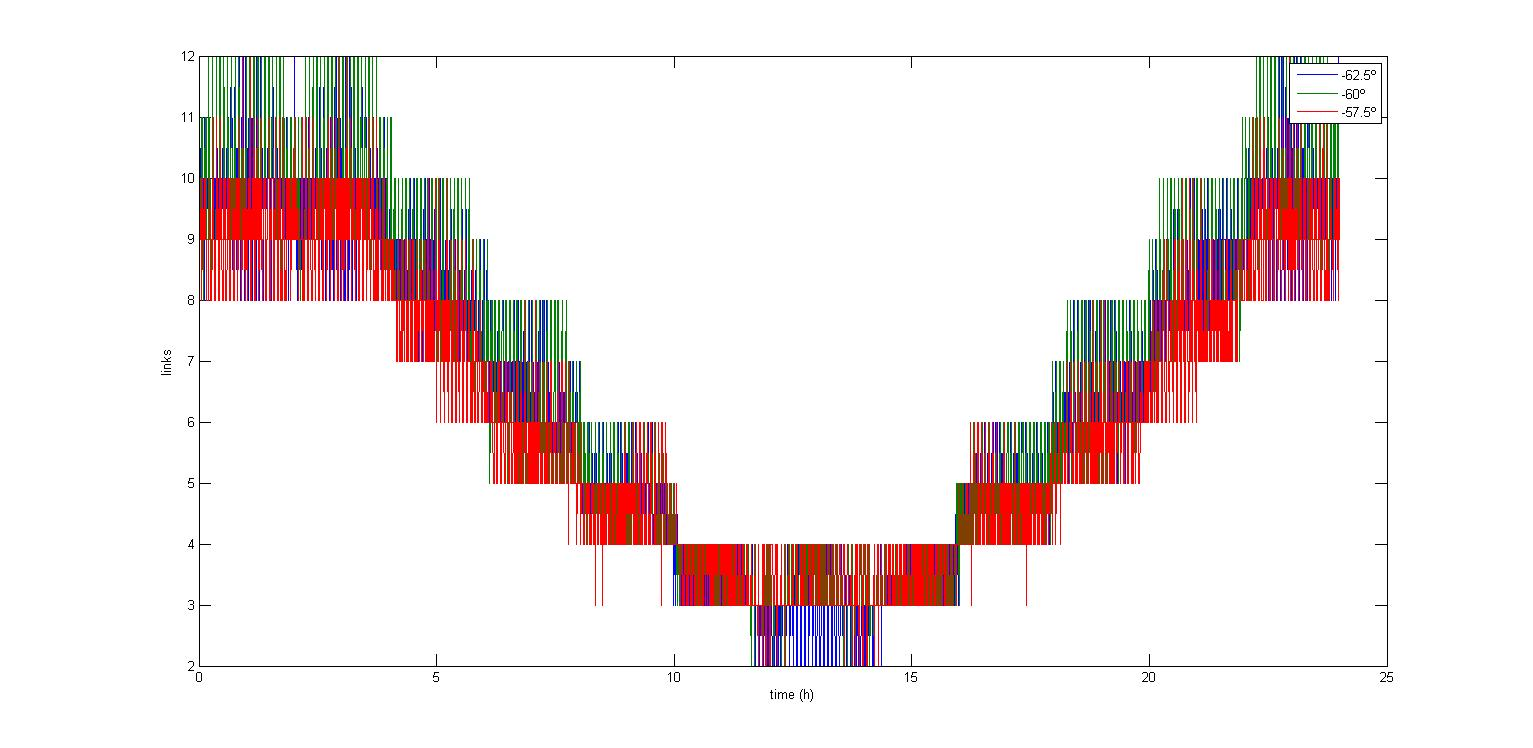
\includegraphics[scale=0.30]{-625_-25_575_(30s)_lat.jpg}
\caption{Links vs time for latitudes from -62.5º to -57.5º with 30 seconds time-step}
\end{center}
\end{figure}

\paragraph{}
In conclusion, the optimum latitudes for the Ground Station are:
\begin{itemize}
\item Between -62.5º and -57.5º
\item Between +57.5º and +62.5º
\end{itemize}

\section{Longitude analysis}
It is intuitive to think that the effect of changing the longitude is delaying the evolution of the coverage. This effect is verified by the algorithm:

\begin{figure}[H]
\begin{center}
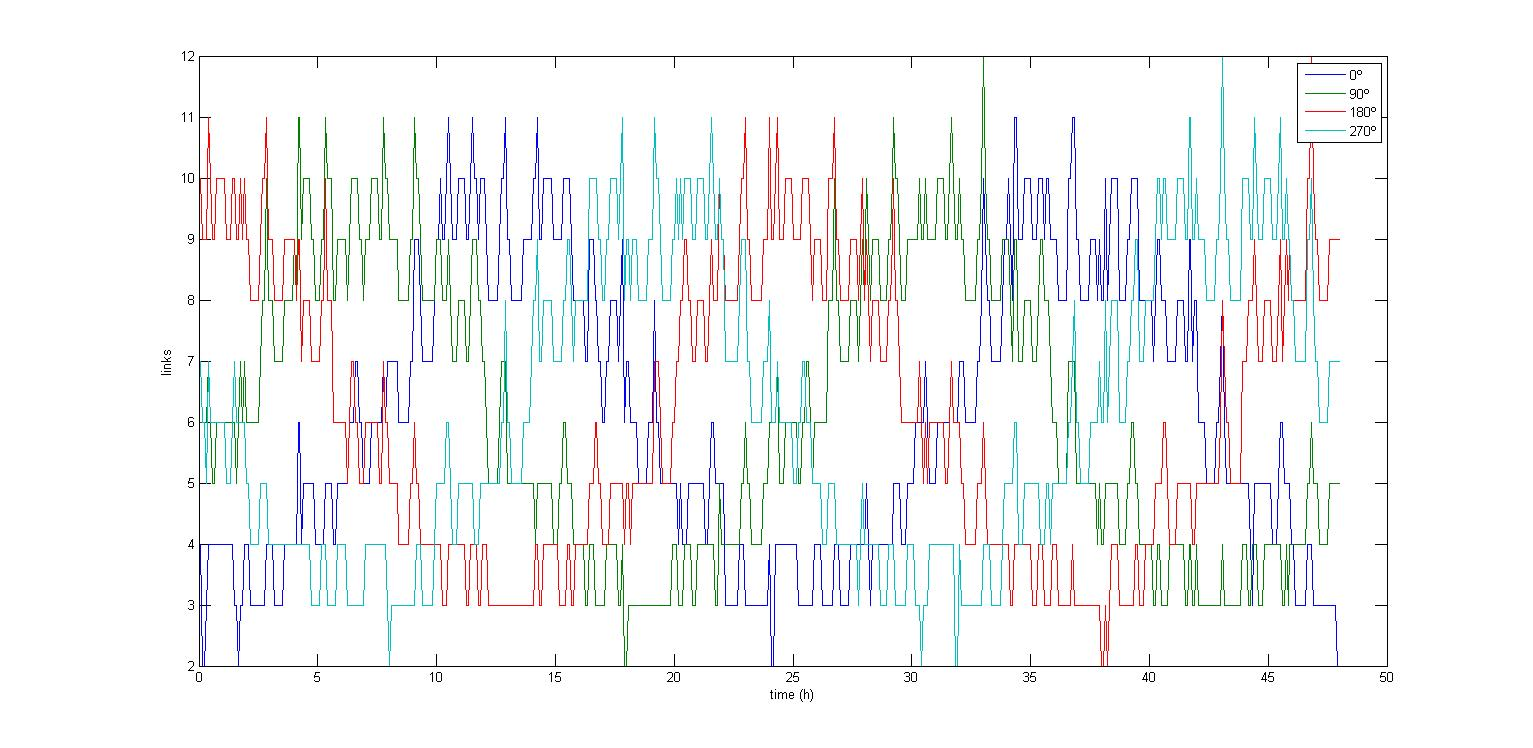
\includegraphics[scale=0.30]{0_90_270_long.jpg}
\caption{Links vs time for longitudes from 0º to 270º}
\end{center}
\end{figure}

\paragraph{}
As it is seen in the figure 1.8 the delay has a reason of 3 hours for every 45º of longitude. 
\paragraph{}
This effect can be used in order to optimize the performance of the Ground Stations. During the day every station will have a peak and a valley in the coverage. Placing the stations with a relative longitude of 120º one to the other would ensure that when one is at the valley other one is at the peak:

\begin{figure}[H]
\begin{center}
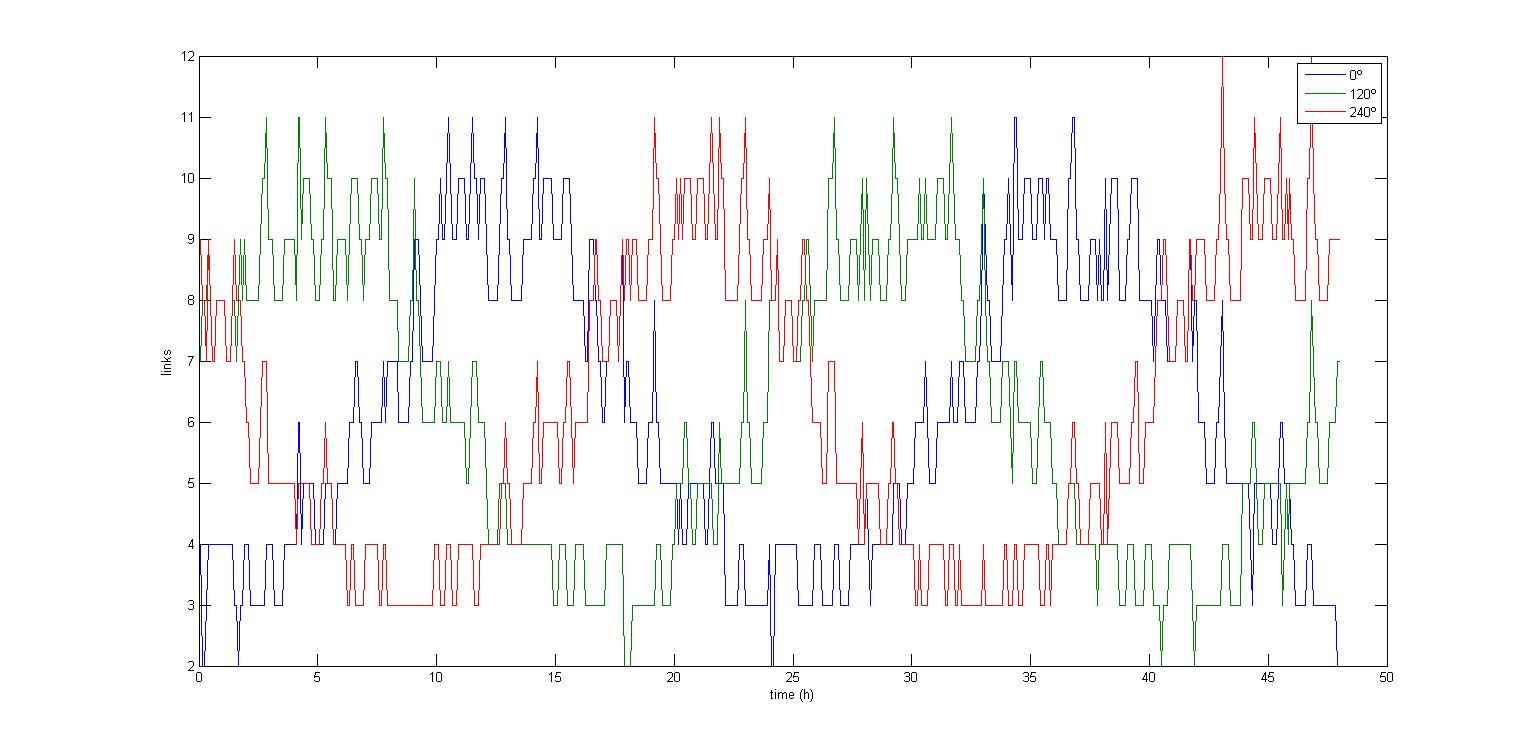
\includegraphics[scale=0.30]{0_120_240_long.jpg}
\caption{Links vs time for longitudes of 0º, 120º and 240º}
\end{center}
\end{figure}

\paragraph{}
In conclusion, the Ground Station should be at a relative longitude of 120º one to the other. It has to be taken in account that this analysis is done for stations at the same latitude. A Ground Station in a given latitude has the same coverage behaviour as an other one at the opposite latitude and 180º of longitude away.
\paragraph{}
To exemplify, the following configurations are equivalent:

\begin{center}
\begin{tabular}{|c|c|c|c|c|c|c|}
\hline 
 & \multicolumn{2}{c|}{GS1} & \multicolumn{2}{c|}{GS2} & \multicolumn{2}{c|}{GS3} \\ 
\hline 
 & Latitude & Longitude & Latitude & Longitude & Latitude & Longitude \\ 
\hline 
Option 1 & 55 & 0 & 55 & 120 & 55 & 240 \\ 
\hline 
Option 2 & -55 & 180 & 55 & 120 & 55 & 240 \\ 
\hline 
Option 3 & 55 & 0 & -55 & 300 & 55 & 240 \\ 
\hline 
Option 4 & 55 & 0 & 55 & 120 & -55 & 60 \\ 
\hline 
Option 5 & -55 & 180 & -55 & 300 & 55 & 240 \\ 
\hline 
Option 6 & -55 & 180 & 55 & 120 & -55 & 60 \\ 
\hline 
Option 7 & 55 & 0 & -55 & 300 & -55 & 60 \\ 
\hline 
Option 8 & -55 & 180 & -55 & 300 & -55 & 60 \\ 
\hline 
\end{tabular}
\end{center}

\section{Conclusion}
\paragraph{}
Summarizing the results of the analysis, for an optimum performance of every Ground Station, they should be at latitudes between -62.5º and -57.5º or between +5.5º and +62.5º. For a better performance of the system every Station should be 120º of longitude away of the other stations if their are at the same latitude or 60º of longitude if they are at the opposite latitude.
\paragraph{}
Taking in account the topography of the Earth there are proposed the following options (every color represent the options for one Ground Station):

\begin{figure}[H]
\begin{center}
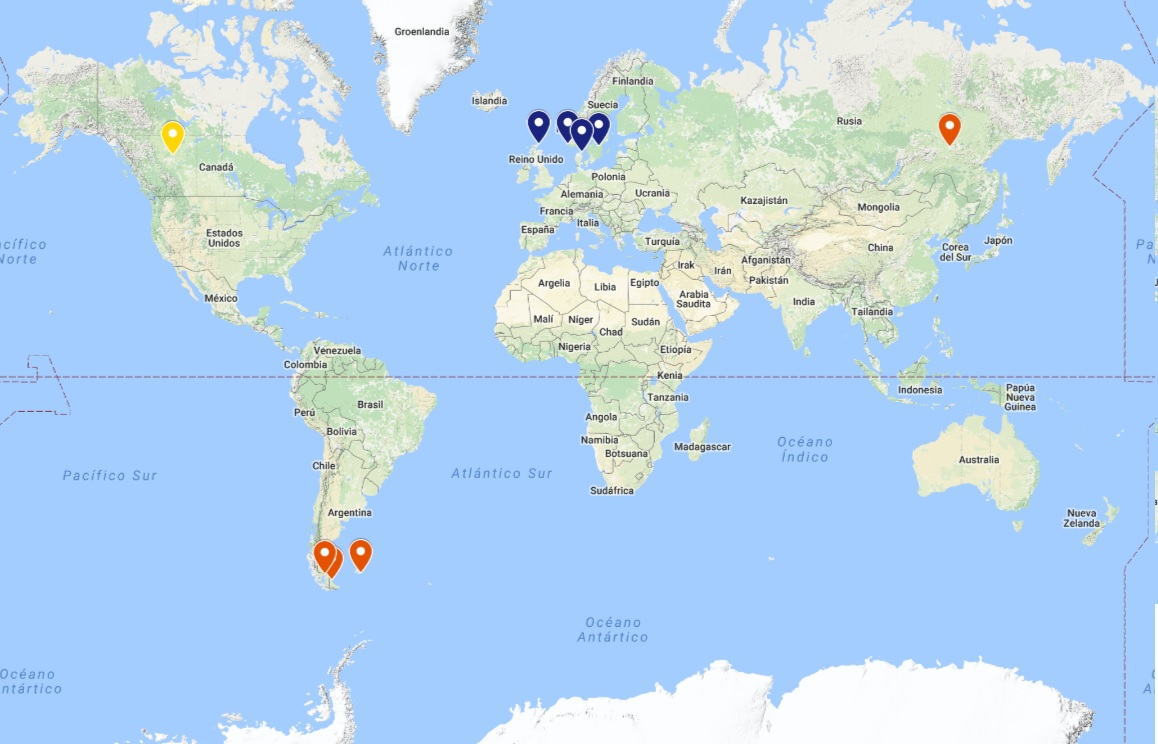
\includegraphics[scale=0.65]{Options.jpg}
\caption{Options for placing the 3 Ground Stations.}
\end{center}
\end{figure}

\paragraph{}
Given this possibilities it has to be done a study of the legislation of the involved countries legislation. The candidate countries are Canada, Argentina, Chile, Falkland Islands (Islas Malvinas), United Kingdom, Denmark, Norway, Sweden and Russia. 

\end{document}